\chapter{Methods}
\label{c:method}

In the following sections, first a number of typical RNA-Seq and DNA-Seq
pipelines that BioCloud supports are defined and explained. Then the design of
BioCloud is explained by breaking down into two main parts: the website and the
report generator. For the website, the components including account
registration, data sources management, experiment design, and pipeline
execution are described and their roles are illustrated in the website overview
workflow. For the report generator, the workflow is shown to demonstrate how
outputs of each tool is extracted, parsed, and rendered into pre-defined
web-based report templates.



\section{RNA-Seq pipelines}
\label{s:rnaseq-pipeline}

The RNA-Seq analysis pipelines that BioCloud supports are summarized in
Figure~\ref{fig:rnaseq-pipeline}, where some of the tools are shared for
different pipelines. The goal of RNA-Seq analysis is to infer differential
expression of gene or transcripts across different conditions. Based on
different assumptions of the distribution of gene and transcript expression,
three different methods are used: Cufflinks, DESeq2, and kallisto, which yield
FPKM based, count-based, and abundance-based expression value respectively.

\begin{figure}[!htbp]
\centering
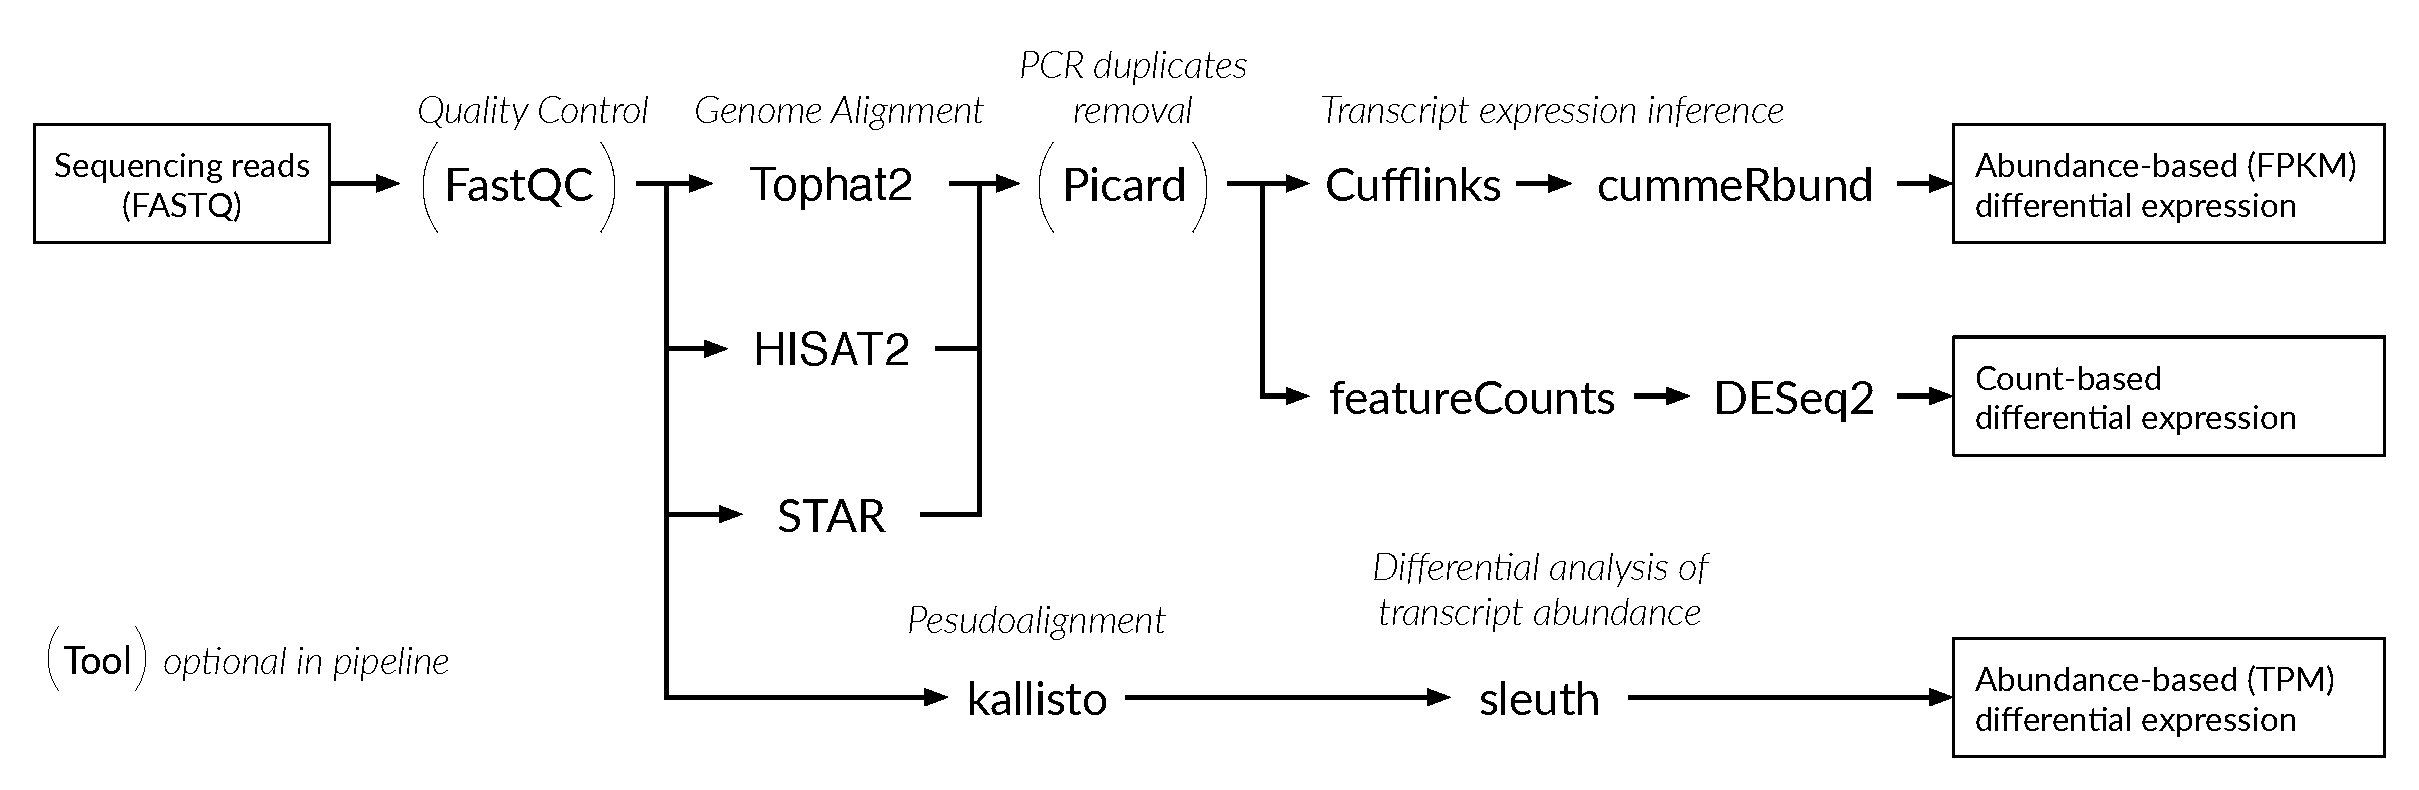
\includegraphics[width=\textwidth]{images/rnaseq_pipelines}
\caption[RNA-Seq analysis pipelines]{RNA-Seq analysis pipelines supported by BioCloud.}
\label{fig:rnaseq-pipeline}
\end{figure}


Cufflinks \cite{trapnell2010:transcript} and its differential analysis method
Cuffdiff \cite{trapnell2013:differential} are best used for gene expression
considering its isoforms, e.g., differential expression on transcript-level.
The output of Cuffdiff can be further visualized using R package cummeRbund
\cite{:cummerbund} from the same development team of Cufflinks. The unit of
expression Cufflinks uses is reads per kilobase of exon per million reads
mapped (FPKM). For DESeq2 \cite{love2014:moderated}, its model analyzes
expression change on gene level using read counts, which cannot be applied to
transcript level analysis. The unit of expression DESeq2 uses is normalized
read counts. The read counts are computed by featureCounts
\cite{liao2014:featurecounts}.  Another popular alternative for computing read
counts is HTSeq \cite{anders2015:htseqa}. HTSeq generally acts the same as
featureCoutns while having slower processing speed so it is not used in
BioCloud.

Both Cufflinks and DESeq2 require genomic location of reads so their analysis
is prepended by the genome alignment step. Three aligners are supported:
Tophat2 \cite{kim2013:tophat2}, HISAT2 \cite{kim2015:hisat}, and STAR
\cite{dobin2013:star}. Though the underlying alignment algorithms of these
tools are different, all of their alignment output in BAM file format can be
used interchangeably by the following expression inference tools. The most
discernible difference is computation time. Given the same execution
environment on a same sequencing sample, Tophat2 takes a hundred times the
computation time of STAR to complete the alignment. HISAT2 uses even slighter
shorter time and significantly less memory than STAR.

Between the genome alignment and expression inference step, an optional step of
removing PCR duplicated reads can be added, which can be done by Picard
\cite{:picard} or Samtools \cite{li2009:sequence}. PCR duplication can occur in
some NGS technology that requires PCR amplification when the given biological
sample has low cDNA template diversity. Filtering out PCR duplication can rule
out the expression bias made by PCR and reduce the computation time due to
fewer reads. However, PCR duplication removal can introduce extra artifact
since no information about PCR duplication can be obtained from the sequencing
data.  That is, the data cannot tell whether a sequence read is PCR duplicated
or not from the sequencing result. Currently the tools label a sequence read as
PCR duplicated if its 5' and 3' genomic position is exactly identical to
another read. Since this empirical rule clamps the dynamic range of gene and
transcript expression, user can choose to skip the step if their NGS technology
does not involve PCR or the PCR duplication effect is negligible.

Contrary to aligning RNA-Seq reads to genome, the concept of pseudoalignment
which does not require actual genome alignment has been brought up in the last
two years. For each sequence read, pseudoalignment finds the most compatible
transcript by sharing the most number of k-mers and use the abundance of k-mers
to infer the estimated the expression of the transcript. By skipping the step
of spliced genome alignment, transcript quantification can be fast and maintain
roughly as accurate as the actual alignment. The idea of pseudoalignment is
first proposed by Salifish \cite{patro2014:sailfish}, formalized and continued
by kallisto \cite{bray2016:nearoptimal} and Salmon \cite{patro2015:accurate}.
Though the differential expression analysis can utilize the existed count-based
analysis tools by rounding the estimated abundance of all transcripts and
summing them to gene level expression, their statistical models on read count
distribution are different. Thus additional tools are developed to provide
better integration with pesudoalignment results, including sleuth
\cite{pimentel2016:differential} and SUPPA \cite{alamancos2015:leveraging}.
Since pseudoalignment is a relatively new concept, only one pipeline is
implemented on BioCloud. User can use kaillisto and sleuth, tools developed by
the same lab, to do pseudoalignment differential expression analysis.

Raw sequence reads are first quality checked using FastQC \cite{:fastqc}.
FastQC provide comprehensive visualization of the quality of sequencing
experiment including per base quality plot, sequencing duplication rate plot,
and adapter sequencing check. FastQC does not affect the content of sequences
thus this step is optional.



\section{DNA-Seq pipelines}

The DNA-Seq analysis pipelines that BioCloud supports are summarized in
Figure~\ref{fig:dnaseq-pipeline}. Some of the tools overlap with RNA-Seq
pipelines which have been already mentioned and described in
Section~\ref{s:rnaseq-pipeline}. To find germline variants, sequence reads are
first aligned to genome by the tool Burrows-Wheeler Alignment (BWA)
\cite{li2009:fast} using its MEM local alignment algorithm.

\begin{figure}[!htbp]
\centering
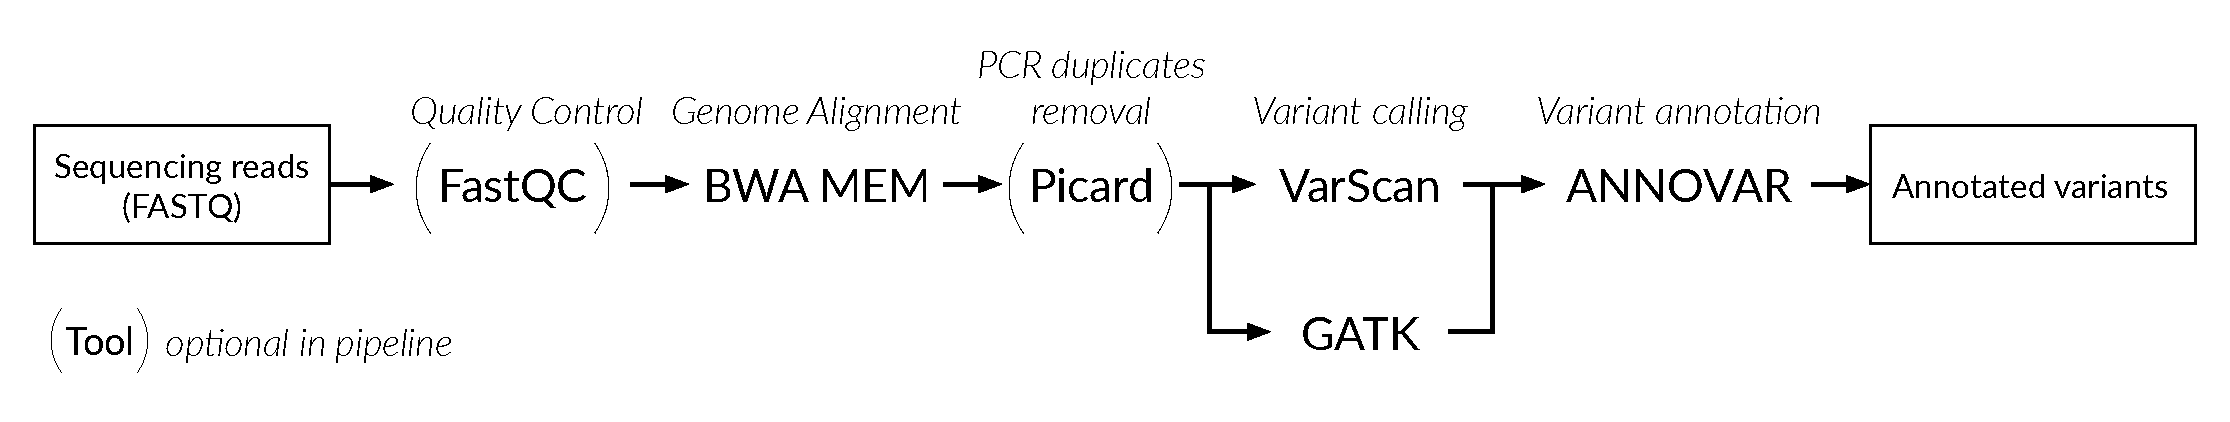
\includegraphics[width=\textwidth]{images/dnaseq_pipelines}
\caption[DNA-Seq analysis pipelines]{DNA-Seq analysis pipelines supported by BioCloud.}
\label{fig:dnaseq-pipeline}
\end{figure}


For variant calling, BioCloud supports two callers: VarScan
\cite{koboldt2012:varscan} and GATK
\cite{vanderauwera2013:fastq,mckenna2010:genome}. To use with VarScan, the
output alignment BAM file is processed by samtools' mpileup subcommand to
compare the aligned reads with genome reference sequence. VarScan take the
mpileup output and determine if it is a significant variant that beyond the
given threshold for each base. To use with GATK, the best practice
\cite{vanderauwera2013:fastq} made by \citeauthor{vanderauwera2013:fastq} is
adopted. However, since our lab does not use GATK for variant calling as
frequently as VarScan, the development to support GATK has been postponed.
Currently existed GATK protocols in our lab are for GATK 1.x, which are
outdated and are not compatible with the newer GATK 2.x.

After variant calling, these variants are further annotated with gene
information, SNP database records, animo acid and protein structure change
predictions by ANNOVAR \cite{wang2010:annovar}. ANNOVAR collects widely used
genome references such as refSeq and Ensembl, annotation databases such as 1000
Genome, dbSNP, ClinVar and COSMIC, and prediction algorithms such as SIFT and
PolyPhen-2. By relying on ANNOVAR, BioCloud don't need to look up each database
and reference on its own, which also reduces the maintaining burden for keeping
all database in use updated.



\section{BioCloud Website}
\label{s:biocloud-website}

In this section, the architecture of BioCloud website is introduced and an
overall picture is given. The workflow for generating summary report is
explained in Section~\ref{s:report-generation}. Except for summary report
generation, the mechanism of each component is explained per subsection,
including a message authentication method for access control and account
validation; experiment design for grouping samples in conditions and is reused
for multiple analyses; analysis submission with parameter settings; job queue;
and finally access control for report and results of an analysis.



\subsection{Overview}

Shown in Figure~\ref{fig:overview-arch}, BioCloud website can be viewed as
three main parts: data storage, computing cluster, and web frontend. For normal
user, they only interact with the web frontend and the architecture of BioCloud
will remain unknown for them. However, in the BioCloud internal structures,
these main parts can exist on different machines. So when large computing
resource is needed, more machines can be added to the computer cluster without
modifying the settings and source code of BioCloud. Data storage includes the
database and local file system to store data sources, genome references and
analysis results and reports. File systems like NFS can be used to allow access
from multiple machines if BioCloud operates across one and more servers.

\begin{figure}[!htb]
\centering
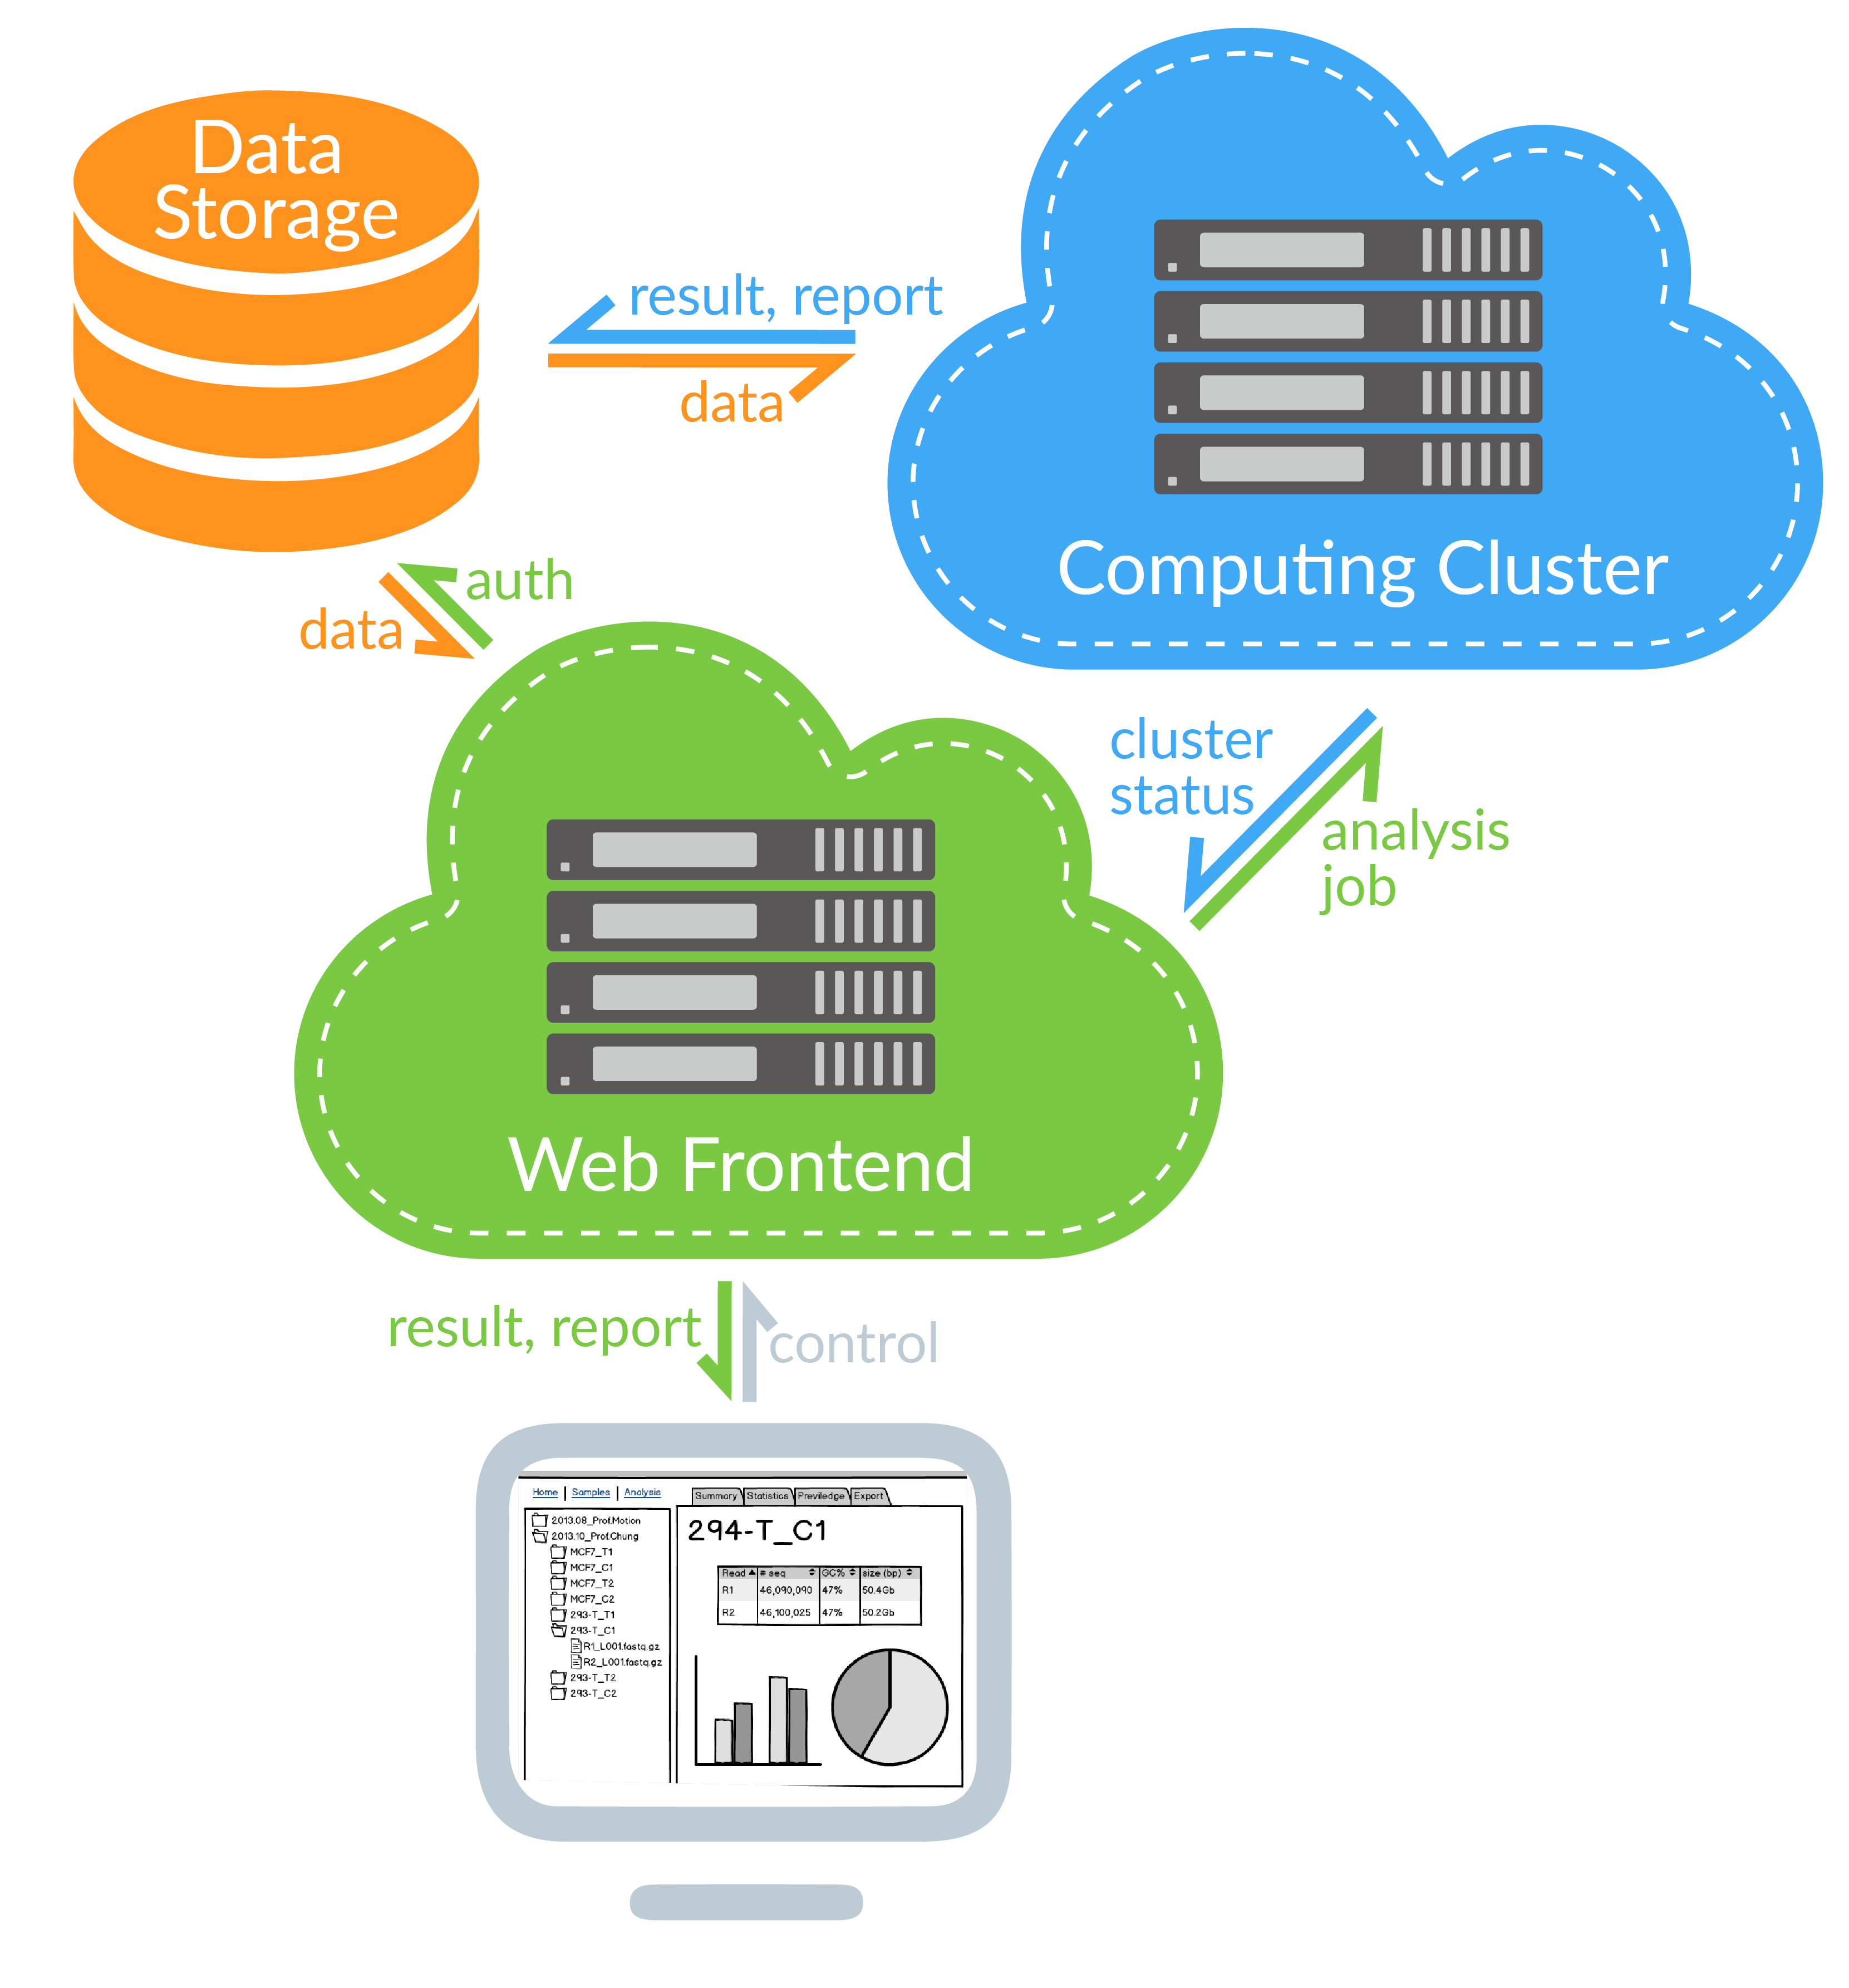
\includegraphics[width=0.75\textwidth]{images/overview_arch}
\caption[BioCloud overview architecture]{Overview of BioCloud architecture.}
\label{fig:overview-arch}
\end{figure}



We further breakdown this general BioCloud architecture into independently
operating components and demonstrate how these components interact in a
workflow of a user completing one analysis in
Figure~\ref{fig:overview-workflow}. Before going down the workflow explanation,
some terminologies BioCloud use should be clarified at first. A data source
represent an file on file system. A sample can be a collection of multiple data
sources. For example, a pair-end sequencing sample contains two data sources
corresponding to the R1 (or forward strand) and the R2 (or reversed strand) of
the sequencing result.

\begin{figure}[!tb]
\centering
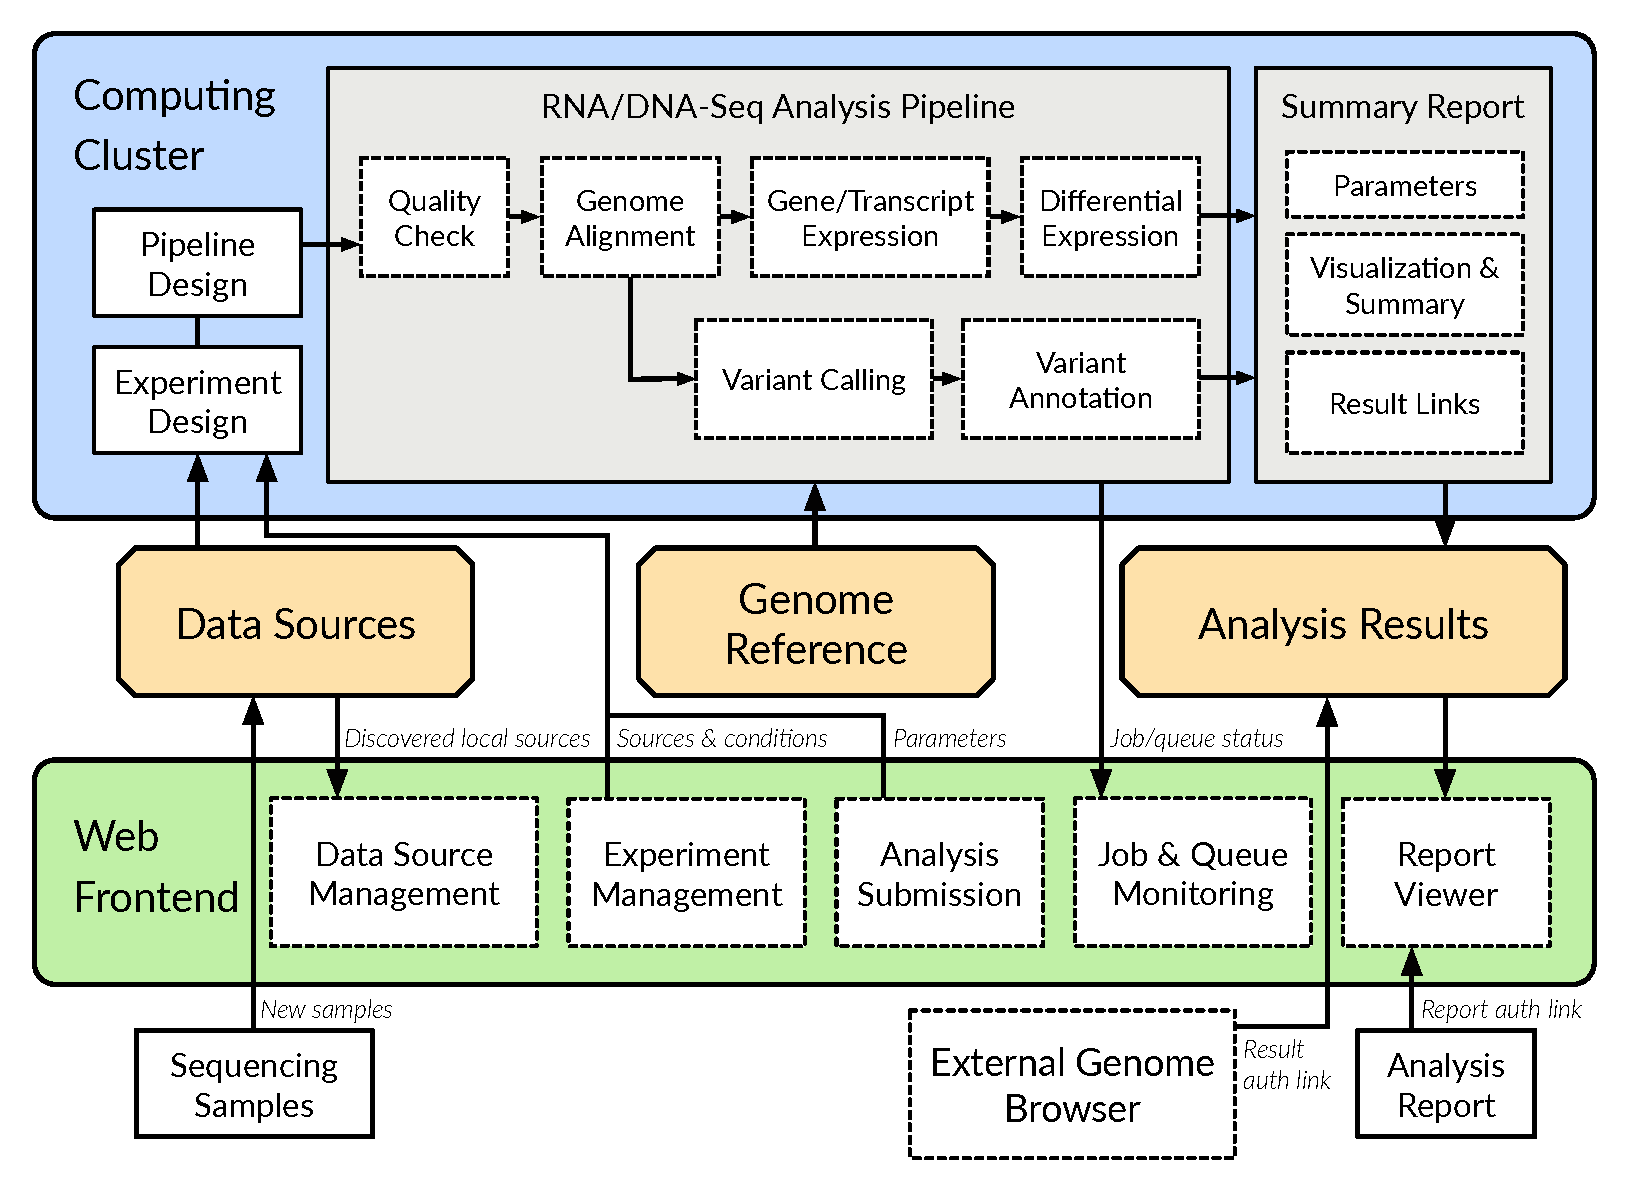
\includegraphics[width=1\textwidth]{images/overview_workflow}
\caption[Overview of BioCloud website workflow]{
    Overview of BioCloud workflow. All operations on data sources, experiments,
    and analysis require user login and thus are isolated by different user
    accounts.
}
\label{fig:overview-workflow}
\end{figure}


The journey of the analysis starts by adding new sequencing samples. These new
samples are added under the user's data source directory. During the auto
discovery, sample name, file type and other information of a source are guessed
by BioCloud but allowed for user to override them. An additional checksum can
be supplied for each source to confirm the data integrity. Data sources or
samples come in group of biological experiments. For example, a experiment can
have control group and test group with 4 samples each. In BioCloud we define
experiment as well, which is a collection of samples. In an experiment, each
selected sample is assigned a condition which can be used for grouping later-on
stages such as differential expression analysis. An experiment can be used in
one and more analyses such as trying different analysis parameters or using
different analysis pipeline. Therefore, an experiment contains which samples to
use and how they are grouped in terms of sample conditions.

Finally, user can now submit an analysis by specifying a pre-defined experiment
and tuning the parameters available for the chosen analysis. User is also
required to select the genome reference used for the analysis, whose possible
options include hg19 (UCSC), hg19 (Ensembl), and hg38 (NCBI). After configuring
and submitting the analysis, the analysis creates its corresponding job and
wait in the job queue for computing cluster to execute. Each analysis pipeline
defines its own unique sequence of execution stages. During the job execution,
the status of these stage reflect either a stage is successfully completed,
failed, running, skipped by user configuration, or waiting for the previous
stage to end. User can obtain the stage status through by monitoring jobs and
the queue. The summary report generation is automatically appended at the end
of each analysis, which is explained in Section~\ref{s:report-generation}. Once
the analysis completes, user will be notified by email with link to the
information page of the analysis.

User can view the summary report by the given link online. Also, outputs of all
executed tools are organized under the folder allocated for this analysis. User
can find the link to download these outputs as well. The report can be shared
to others without a BioCloud account by simply sharing the link. The link to
results and report can be set as private access or have a new URL if user does
not want to disclose their report and result anymore. By pasting the link to
results on genome browser like Ensembl and UCSC, user can immediately view
their results with other genome annotations without uploading full output file
to the genome browser.

\begin{figure}[htbp]
\centering
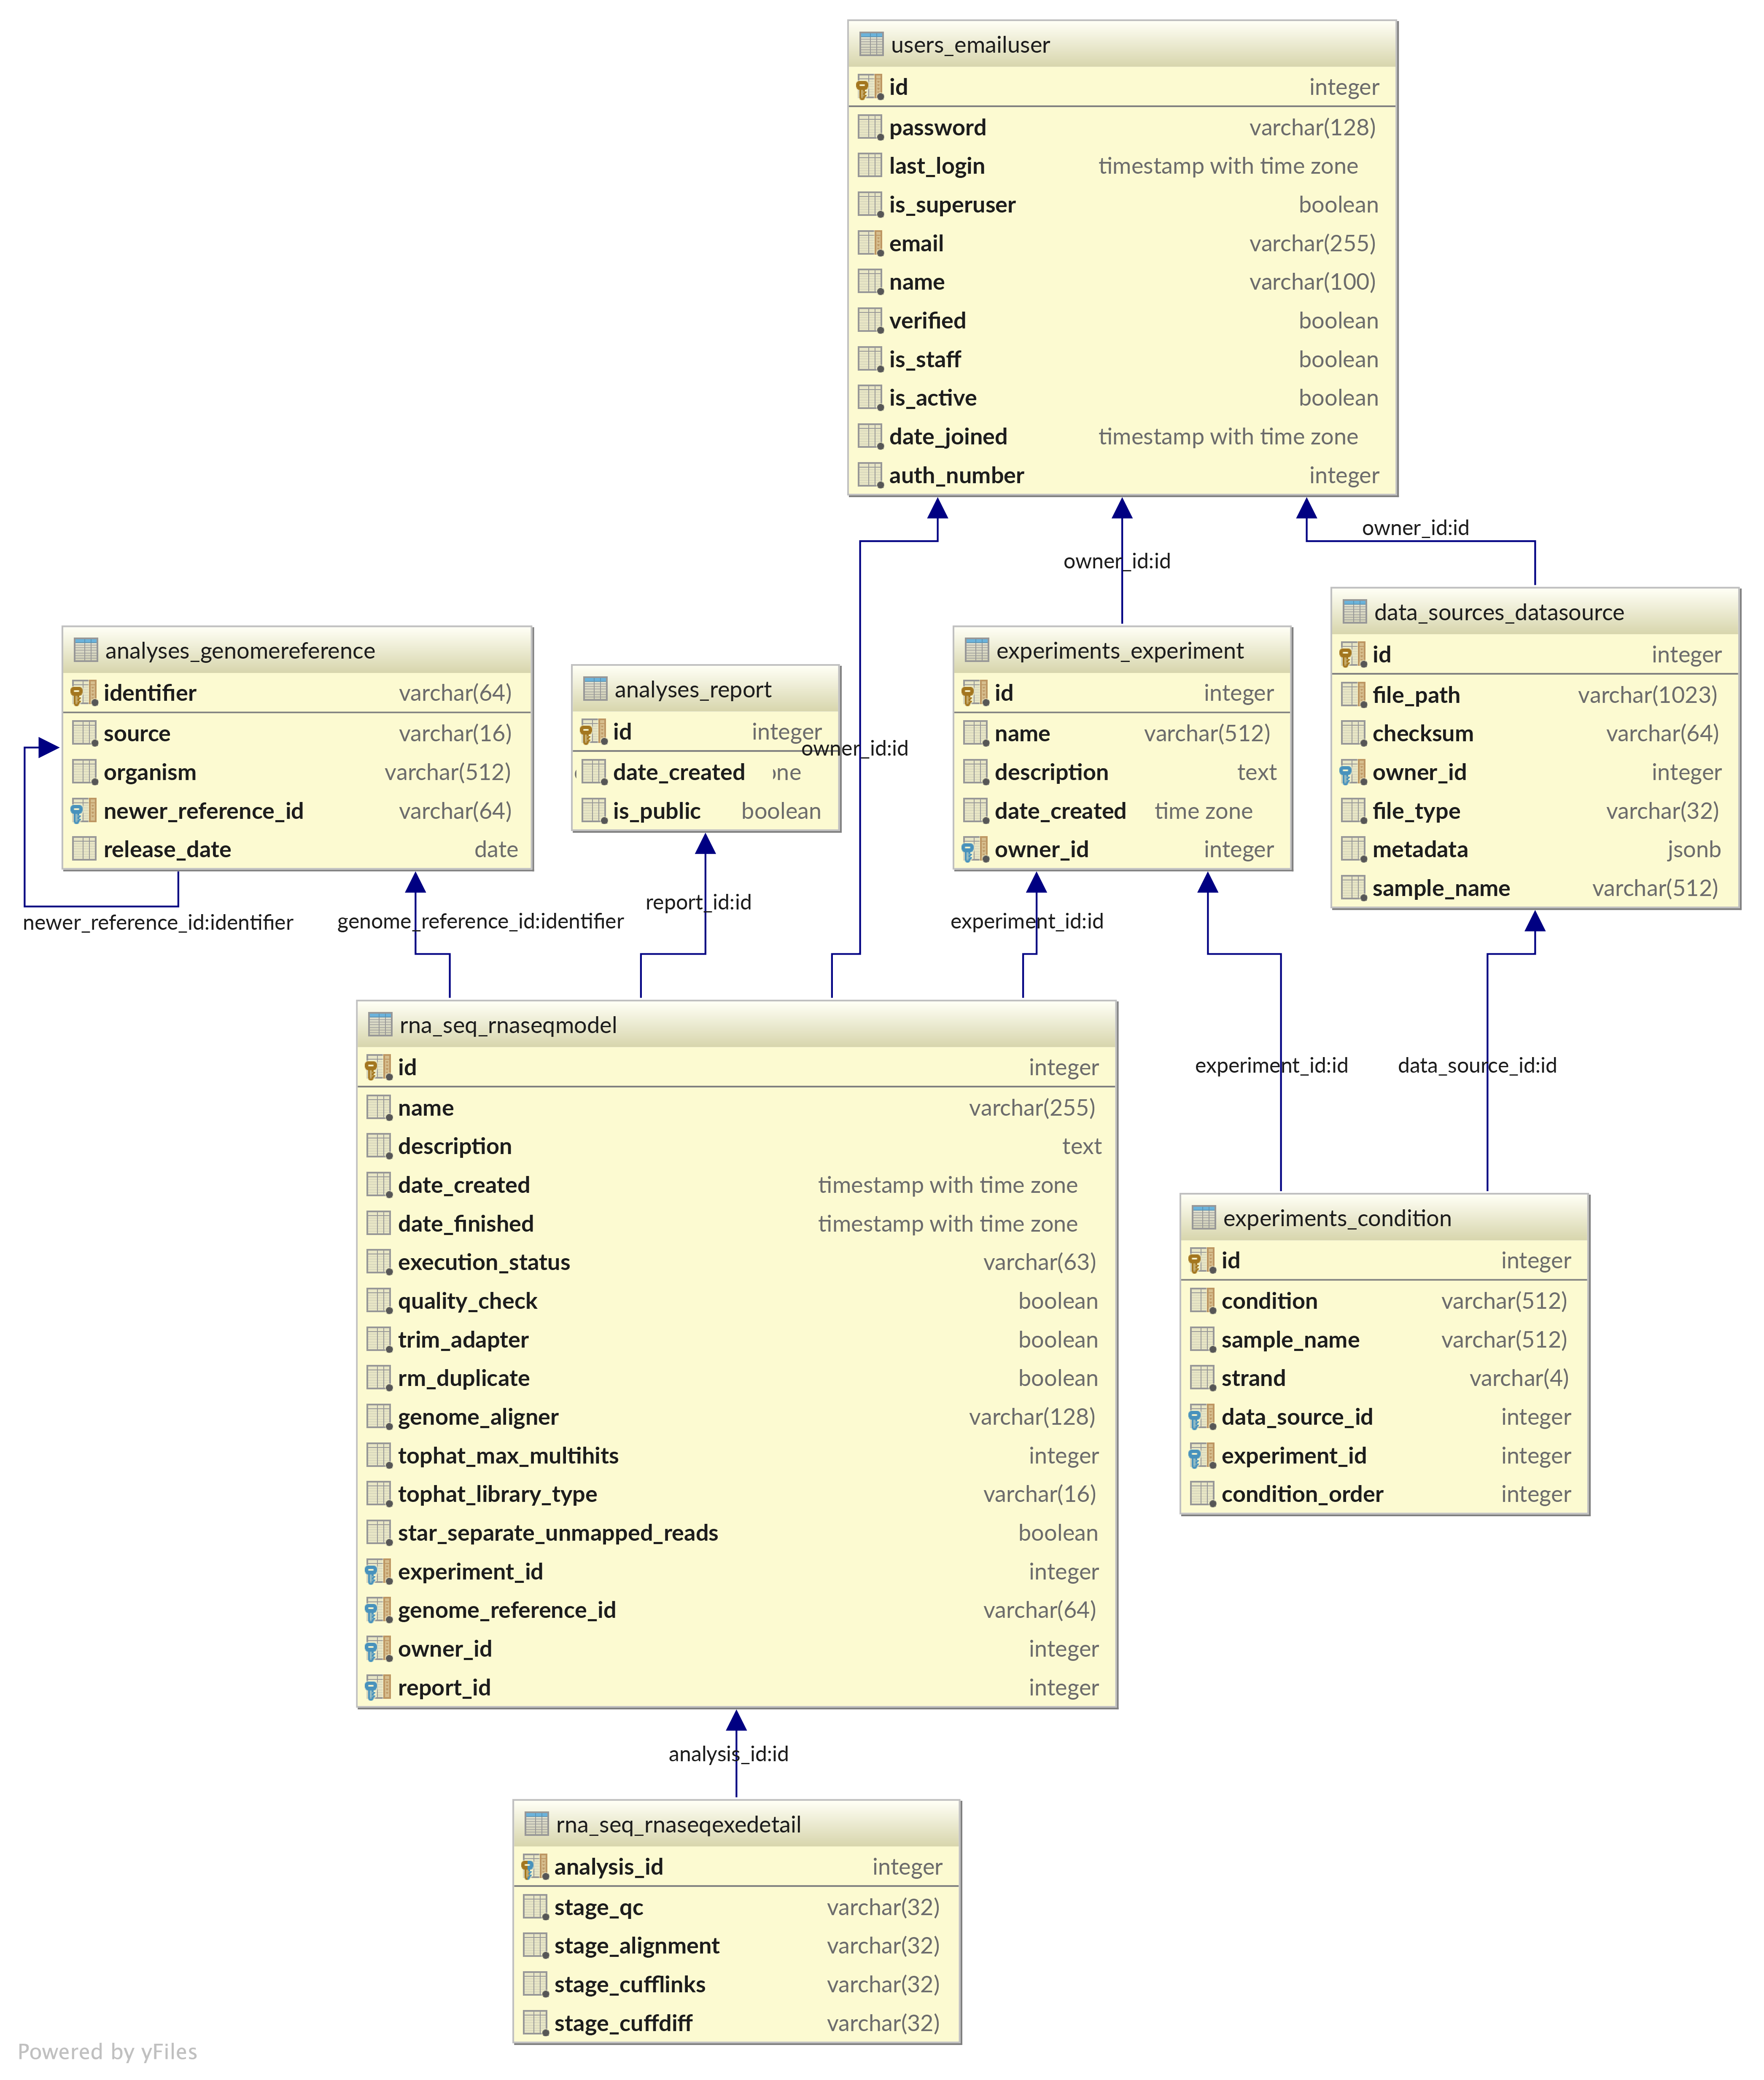
\includegraphics[width=\textwidth]{images/biocloud_erd}
\caption[Entity relation diagram (ERD) of BioCloud database]{
    Entity relation diagram (ERD) of BioCloud database. Here only one analysis
    pipeline of RNA-Seq (table \texttt{rna\_seq\_rnaseqmodel}) is shown for
    simplicity. Tables related with Django web framework internals and job
    queue framework are also omitted.
}
\label{fig:biocloud-erd}
\end{figure}


So far all major components of BioCloud have been covered and they will be
explained in detail in the following subsections. The corresponding database
design is shown in Figure~\ref{fig:biocloud-erd}.


\subsection{Data integrity check and authentication}

Data integrity check and authentication are important topics in BioCloud
website. Data sources need to be checked if the content of uploaded file is
identical to that of user's local copy. During account activation, an unique
activation link for this account is generated and sent to the email registered
by the account. When the user clicks the link, BioCloud knows which account is
activated and is certain that user actually posses this email address. For
sharing report or result through given link, BioCloud verify the link is valid
and retrieve the corresponding analysis report or result. Except for data
integrity check, we have to make sure all the links mentioned above cannot be
forged in a reasonable time given the current computing power. Therefore, in
BioCloud several methods are used to make sure the data integrity and to
validate authentication link and code.

To check data integrity of upload data sources, a checksum per file using
SHA2-256 hash algorithm can be passed during the data source discovery can be
provided. Checksum summarizes the file into a fixed length of bits no matter of
the file size. The checksum algorithm is sensitive to minor changes, so if a
file have a few bytes corrupted during the network transmission, its checksum
will be drastically different to the correct counterpart. Checksum is not file
compression so it can only be used for data integrity check. The checksum of
two different files can be identical, the incident being referred to as
collision. The checksum algorithm in use, SHA2-256, generates 256bits long
checksum.

For authentication, hash-based message authentication code (HMAC) is used to
create the authentication key. A HMAC string consists of two parts: the
original message and a signature for the original message, which is generated
with a secret key and a salt string in the current BioCloud implementation. The
signature is a hash is generated based on the given secret key concatenating to
salt string and the original message. Since the secret key is not disclosed to
user, knowing the original message and the salt string cannot re-create the
signature. The only way to forge the signature is through hash collision.
However, by choosing cryptographic hash function such as SHA-1\footnote{
    SHA-1 is not considered collision resistant anymore, though it is still
    suitable to be used as the hash function of HMAC.
} and SHA-2, they are collision resistant so it is hard to find a collision
in feasible time. The salt key, public or private, extends the computation
effort to crack the underlying secret key. By passing JSON as the original
message, one can store complex data structure in one HMAC string.


\subsection{User account management}

To let individuals manage their own data sources, analyses and results,
BioCloud builds its user account management based on Django's implementation.
Security is one of the top concern for BioCloud, we rely on the password
management made by Django which is secure and long tested in the public.
BioCloud requires email and password for registration.

Since it sends out email notification to users, the email address is first
verified by sending an activation link upon registration. The link contains a
HMAC token consisting of user's email address and registration timestamp. The
timestamp can verify if the activation link has been expired. The activation
link is generated on-the-go when a user requests. Compared to alternative
solution to store activation links in the database, our approach does little
performance impact on database system. A user is marked as verified once the
account activation is complete.

To better maintain the BioCloud, special account types, staff and superuser
account, can access to the BioCloud admin interface and view and modify all
users' data and activities. Superuser doesn't need to permission to do all
operations in the admin interface, whereas staff can only performance a subset
of granted operations. The account type can be adjusted by
\texttt{is\_superuser} and \texttt{is\_staff} columns of
\texttt{users\_emailuser} table, as shown in Figure~\ref{fig:biocloud-erd}.
User's data sources and experiments, and analyses are referred back to its user
record via \texttt{owner\_id} column on their respective table.


\subsection{Data source management}

Once the account is initiated, BioCloud create a folder for user to store
data sources based on the user ID. User ID is auto generated and unique. User
can either move or link their data sources under this folder.

User then add these data sources using ``data source discovery'' function of
BioCloud. It scans user's data source folder and filter newly added sources
with the user's database records. Sample name and type of the data source is
guessed by BioCloud. After the discovery, user can override the guessed values
and add checksum for each discovered files. User can later change these
property after the data sources are added as well.

The representation of data source in the database is a straight-forward
mapping, as table \texttt{data\_sources\_datasource} shown in
Figure~\ref{fig:biocloud-erd}. However, there are some metadata that are only
required for certain file types. For example, only FASTA and FASTQ files can be
pair-end, e.g., R1 and R2. Metadata is stored as a column of JSON type.
Metadata can be a hierarchical data structure in one column and database won't
complain if some substructure of a metadata record cannot be found in another.


\subsection{Experiment design}

Experiment collects a group of data sources and labels them with conditions. An
example of experiment design is shown in Table~\ref{tab:experiment-example}. In
this experiment, four samples, A, B, C and D, from user ID 1 with pair-end
FASTQ files, are selected. The former two samples are of condition control,
while rest of the samples are of condition testing.

\begin{table}[!htb]
    \caption[Example of experiment design]{Example of experiment design.}
    \label{tab:experiment-example}
    \centering
    \begin{threeparttable}
        \begin{tabular}{ccrr}
            \toprule
            Condition & Sample name & Forward read (R1) & Reversed read (R2) \\
            \midrule
            Control & A & \texttt{1/A\_1.fastq} & \texttt{1/A\_2.fastq} \\
            Control & B & \texttt{1/B\_1.fastq} & \texttt{1/B\_2.fastq} \\
            Testing & C & \texttt{1/C\_1.fastq} & \texttt{1/C\_2.fastq} \\
            Testing & D & \texttt{1/D\_1.fastq} & \texttt{1/D\_2.fastq} \\
            \bottomrule
        \end{tabular}
    \end{threeparttable}
\end{table}


BioCloud creates an interactive frontend for user to filter and select the data
sources they want to include in this experiment. Since a simple may have
multiple data sources, by default BioCloud guesses using the sample information
during discovery. However, user can override the sample name during experiment
design. For example, user can create a new sample called AC and include all
four data sources originally of sample A and C. After finalizing the samples,
user defines the available conditions for this experiment and assign sample to
them.

To sum up, there are three steps to design an experiment: select data sources,
label sample name on data sources, label condition on samples. However, user
can freely go back and modify result of the previous stage. BioCloud will try
to re-use all user given information maximally as possible so user don't need
to re-fill all the information again. For example, if the condition ``Control''
is misspelled as ``Contorl'', when updating the condition name, all samples of
the condition will remain and their condition names will be updated
simultaneously. BioCloud achieves this feature by binding condition and sample
name only on data sources' metadata, and user updates directly to the metadata.
When a metadata is changed, BioCloud decides which part of the experiment
design is changed and re-renders all the affected output. This is the notion of
web frontend development called reactive programming.

User can give experiment name and description to help manage all defined
experiments. Description is written in Markdown syntax \cite{:commonmark},
which is a lightweight markup language that convert plain texts into styled
document. Users are encouraged to put relevant links and references regarding
to the experiment in its description.


\subsection{Genome reference}

\subsection{Analysis submission}

\subsection{Job queue management}

\subsection{Report and result access control}



\section{Report generation}
\label{s:report-generation}

\subsection{BCReport: result processing framework}



\section{Implementation}

\subsection{Website}


% database
BioCloud code base communicates with the database via Object-relational Mapping
(ORM), which continually checks with consistency between the database scheme
and the mapped object representation in source code.


\subsection{Deployment}

\subsection{Report}
% vim: set textwidth=79:
